\chapter{Introduction\label{cha:chapter1}}
Due to significant amount of new Missions, German Orbital System took a step up to create a type of satellite bus for 6U satellite.  As a result of updating the bus from 3U to 6U, satellite functions have improved, which opens up the possibility for more subsystems and components, as well as for payloads. The configuration of the separate power distribution unit made it possible to place more components on which the number of working subsystems and payloads increased. Development process of the satellite including EPS is taking a sizable amount of time, to use time more efficient was decided to divide the EPS in to two units and create an universal Power Distribution Unit which is admissible for 6 Unit as well as for a 3 Unit CubeSats. 
 

\section{Motivation\label{sec:moti}}
Nowadays most of the companies designing their Electrical Power System boards for a nano cubesats as whole unit, consisted of all important devices for power management. This configuration is common and allowed to create space for a hardware in the tiny cubesat which is essential for a nano satellites due to its limited size and mass. 
\\  Despite the fact that mechanical space of the satellite is important, the space on the EPS board is limited for a components which is narrowing satellite possibilities with bigger missions and more developed bus. 
The motivation of this research is to find the optimal solution of the Power Distribution Unit architecture of Electrical Power System for the 6U CubeSat. Development of Power Distribution Unit will make a responsible use of time for a next missions, by development only a Power Processing Unit, which will be configured for each mission individually.

\section{Objective\label{sec:objective}}

One unit configuration is a common type of an EPS design, which is mostly used by nano cubesat developers. This type of EPS design allowed to combine all components of the EPS in one unit to save mechanical space for the rest of the bus hardware and a payload of a nano cubesat. Second type of technology is a separated type of the EPS which is divided in to PPU which is responsible for a power generation from a solar panels, battery charging and balancing as well as power processing and power convertation and PDU which has a function of the power distribution. PDU consist mostly of switchers and current sensors, this architecture allowed to place significant amount of switchers and connectors for a payloads, which are necessary for a missions requiring amount of payload connections which will not be enough for a standard one unit EPS board type. \\

\section{Scope\label{sec:scope}}

Here you should describe what you will do and also what you will not do. Explain a little more specific than in the objective section. 'I will implement X on the platforms Y and Z based on technology A and B.'

Conclude this subsection with an image describing 'the big picture'. How does your solution fit into a larger environment? You may also add another image with the overall structure of your component.

'Figure \ref{fig:intro} shows Component X as part of ...' 
\\
\begin{figure}[htb]
  \centering
  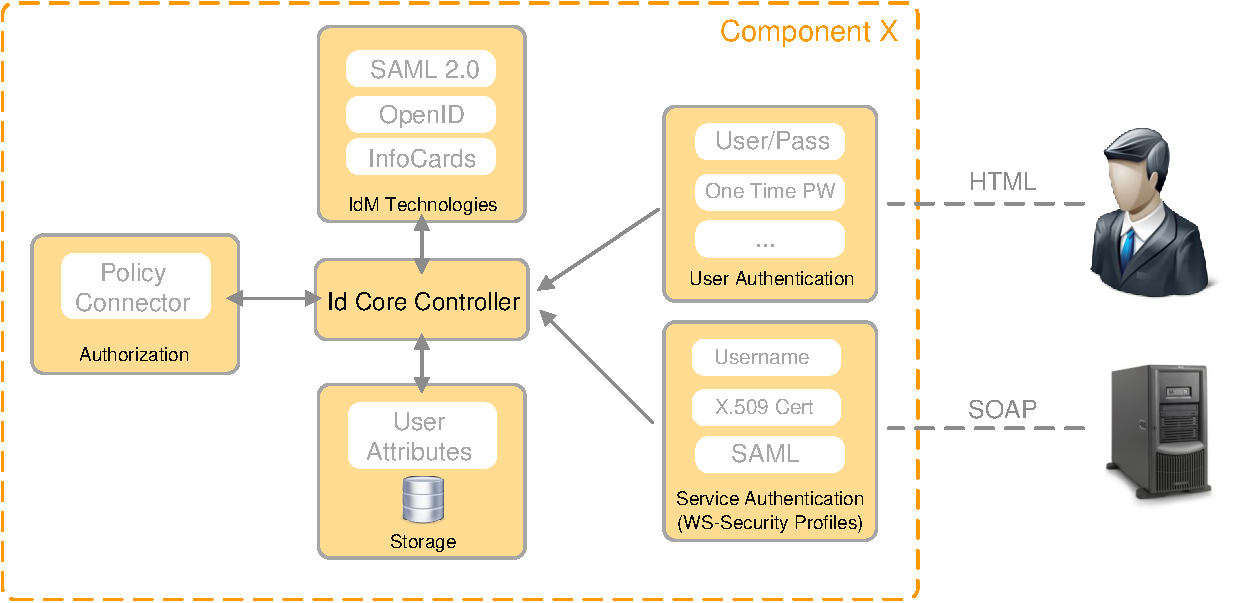
\includegraphics[width=9cm]{intro_example.pdf}\\
  \caption{Component X}\label{fig:intro}
\end{figure}

\section{Outline\label{sec:outline}}

The 'structure' or 'outline' section gives a brief introduction into the main chapters of your work. Write 2-5 lines about each chapter. Usually diploma thesis are separated into 6-8 main chapters. 
\\
\\
\noindent This example thesis is separated into 7 chapters.
\\
\\
\textbf{Chapter \ref{cha:chapter2}} is usually termed 'Related Work', 'State of the Art' or 'Fundamentals'. Here you will describe relevant technologies and standards related to your topic. What did other scientists propose regarding your topic? This chapter makes about 20-30 percent of the complete thesis.
\\
\\
\textbf{Chapter \ref{cha:chapter3}} analyzes the requirements for your component. This chapter will have 5-10 pages.
\\
\\
\textbf{Chapter \ref{cha:chapter4}} is usually termed 'Concept', 'Design' or 'Model'. Here you describe your approach, give a high-level description to the architectural structure and to the single components that your solution consists of. Use structured images and UML diagrams for explanation. This chapter will have a volume of 20-30 percent of your thesis.
\\
\\
\textbf{Chapter \ref{cha:chapter5}} describes the implementation part of your work. Don't explain every code detail but emphasize important aspects of your implementation. This chapter will have a volume of 15-20 percent of your thesis.
\\
\\
\textbf{Chapter \ref{cha:chapter6}} is usually termed 'Evaluation' or 'Validation'. How did you test it? In which environment? How does it scale? Measurements, tests, screenshots. This chapter will have a volume of 10-15 percent of your thesis.
\\
\\
\textbf{Chapter \ref{cha:chapter7}} summarizes the thesis, describes the problems that occurred and gives an outlook about future work. Should have about 4-6 pages.